\section{Mantel-Haenszel Chi-Squared Test}
In the $i$-th table, given the marginal totals $n_{1,i}$, $n_{2,i}$, $n_{.1,i}$, $n_{.2,i}$ are fixed, the random variable $n_{11,i}$ has a hyper-geometric distribution.
\[\P(n_{11,i} = z) = \frac{{n_{1,i} \choose z} {n_{2,i} \choose n_{.1,i} - x}}{{n_i \choose n_{.1,i}}}.\]

Under the $H_0$, we have
\begin{align*}
	\E (n_{11, i}) =& \frac{n_{1,i}n_{.1,i}}{n_i};\\
	\Var (n_{11,i}) =& \frac{n_{1,i}n_{2,i}n_{.1,i}n_{.2,i}}{n_i^2 (n_i - 1)}\\
\end{align*}

Also under the $H_0$, we have the statistic $\operatorname{MH}$ for Mantel-Haenszel Chi-squared Test.
\[\operatorname{MH} = \frac{\sum_{i=1}^{i}(n_{11,i} - \E (n_{11,i}))}{\sqrt{\sum_{i=1}^{i} \Var( n_{11,i})}}\]

The rejected regions are as follows.
\begin{figure}[H]
	\centering
	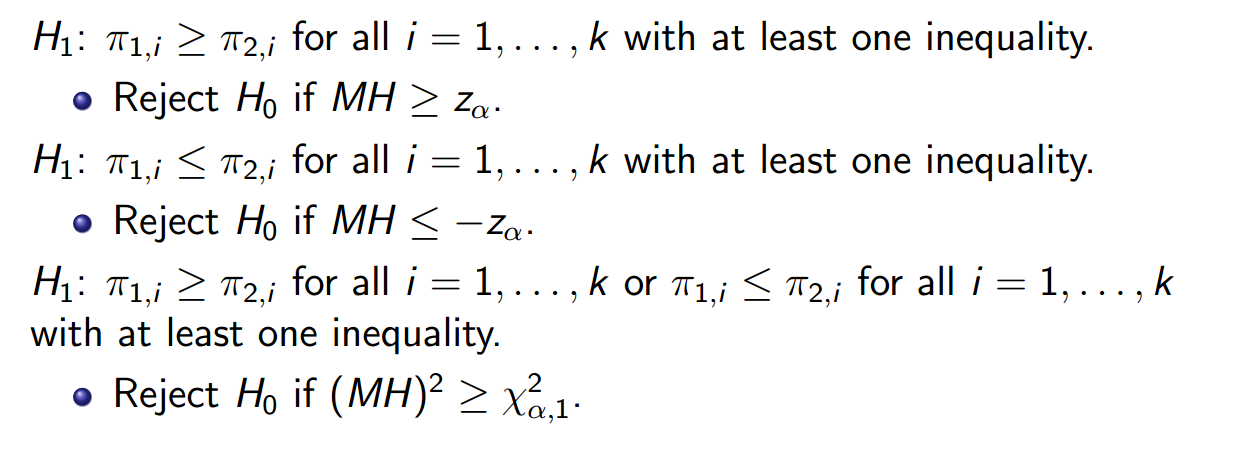
\includegraphics[width=0.7\linewidth]{fig/screenshot007}
	\caption{Rejected Region}
	\label{fig:screenshot007}
\end{figure}

\subsection{Example 1}
\lstinputlisting[language=R]{code/l11-exp3.R}

\subsection{Example 2}
Transform the data if it is not categorical.
\lstinputlisting[language=R]{code/l11-exp4.R}

